\documentclass[]{ximera}
%handout:  for handout version with no solutions or instructor notes
%handout,instructornotes:  for instructor version with just problems and notes, no solutions
%noinstructornotes:  shows only problem and solutions

%% handout
%% space
%% newpage
%% numbers
%% nooutcomes

%I added the commands here so that I would't have to keep looking them up
%\newcommand{\RR}{\mathbb R}
%\renewcommand{\d}{\,d}
%\newcommand{\dd}[2][]{\frac{d #1}{d #2}}
%\renewcommand{\l}{\ell}
%\newcommand{\ddx}{\frac{d}{dx}}
%\everymath{\displaystyle}
%\newcommand{\dfn}{\textbf}
%\newcommand{\eval}[1]{\bigg[ #1 \bigg]}

%\begin{image}
%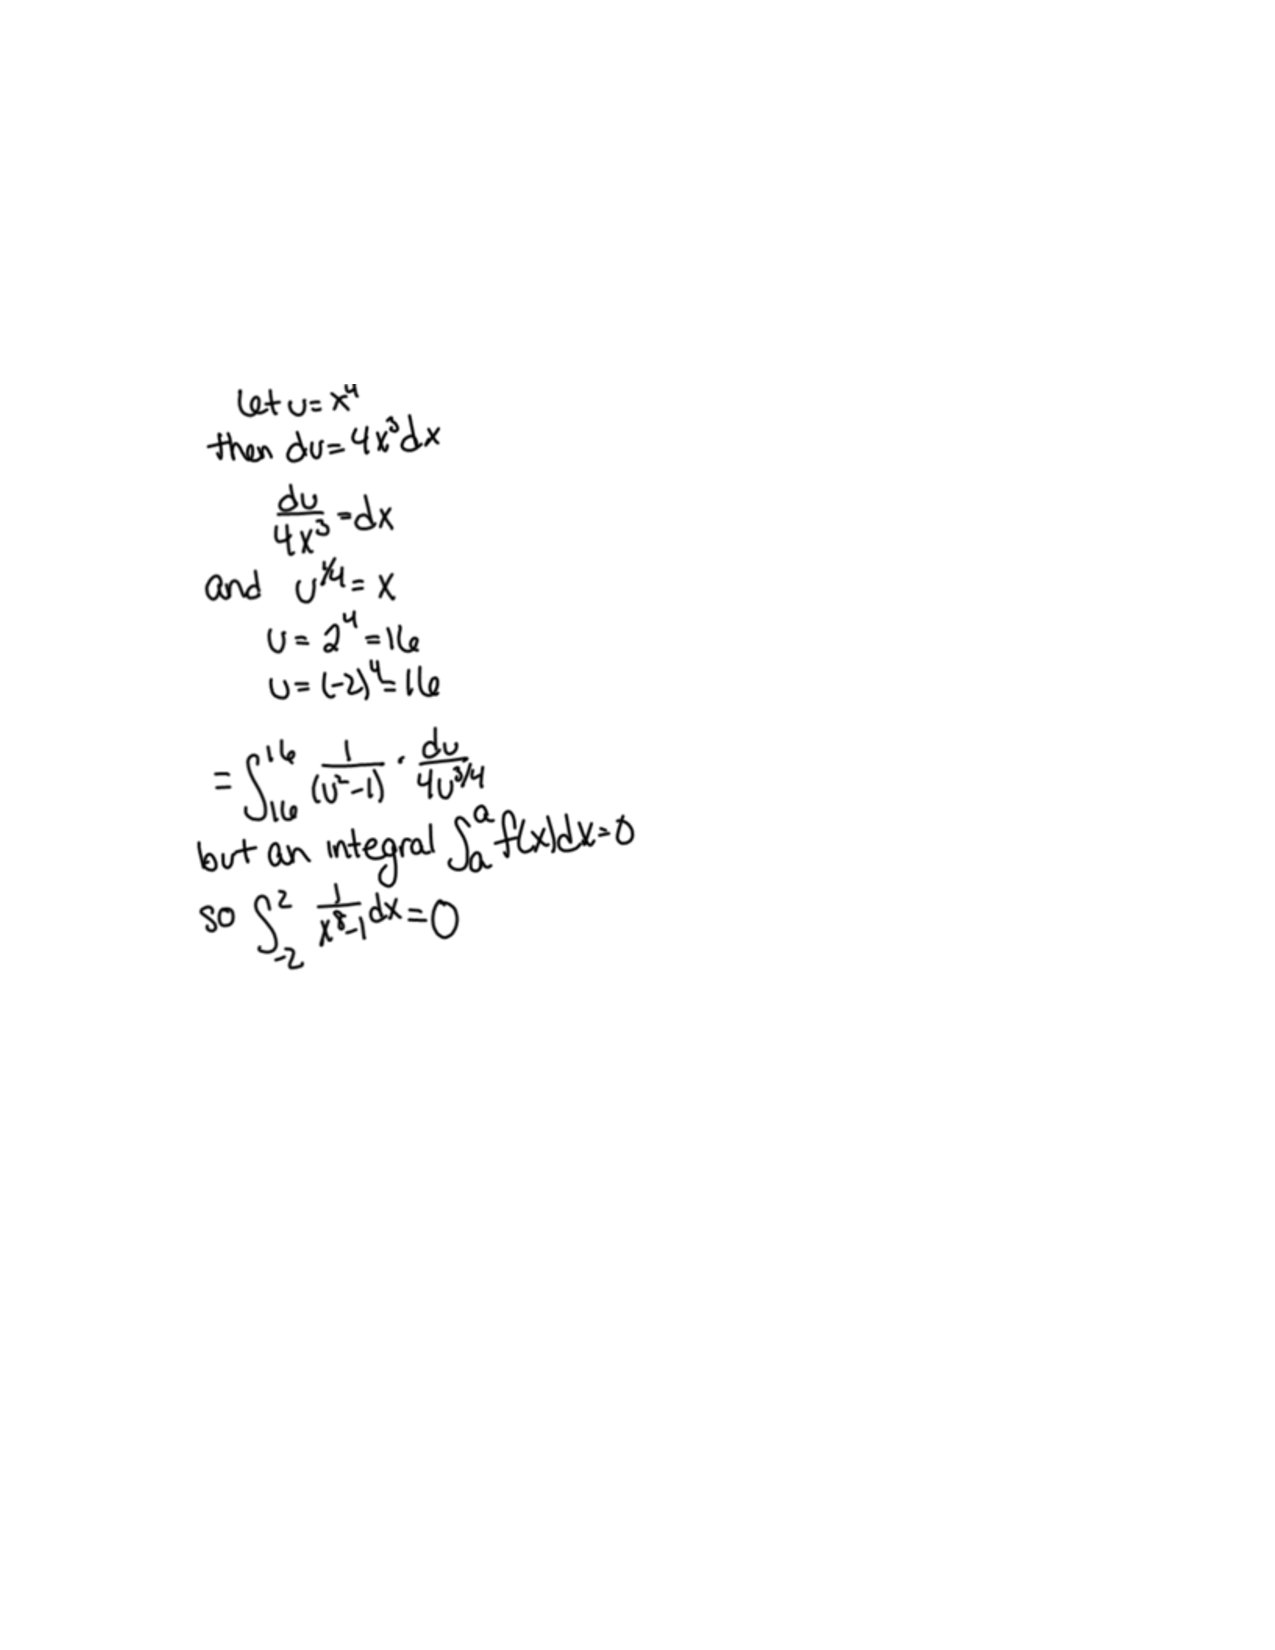
\includegraphics[trim= 170 420 250 180]{Figure1.pdf}
%\end{image}

%add a ``.'' below when used in a specific directory.
\newcommand{\RR}{\mathbb R}
\renewcommand{\d}{\,d}
\newcommand{\dd}[2][]{\frac{d #1}{d #2}}
\renewcommand{\l}{\ell}
\newcommand{\ddx}{\frac{d}{dx}}
\newcommand{\dfn}{\textbf}
\newcommand{\eval}[1]{\bigg[ #1 \bigg]}

\usepackage{multicol}

\renewenvironment{freeResponse}{
\ifhandout\setbox0\vbox\bgroup\else
\begin{trivlist}\item[\hskip \labelsep\bfseries Solution:\hspace{2ex}]
\fi}
{\ifhandout\egroup\else
\end{trivlist}
\fi} %% we can turn off input when making a master document

\title{Properties of power series}  

\begin{document}
\begin{abstract}		\end{abstract}
\maketitle



\section{Warm up:}
Suppose that $\sum_{k=0}^\infty c_k (x+5)^k$ converges when $x=-9$ and diverges when $x=-1$.  
What can be said about the convergence and divergence of the following series?
	\begin{multicols}{3}
	\begin{enumerate}
	\item  $\sum_{k=0}^\infty c_k$
	\item  $\sum_{k=0}^\infty c_k (-5)^k$
	\item  $\sum_{k=0}^\infty c_k (5)^k$
	\end{enumerate}
	\end{multicols}
	
	\begin{freeResponse}
	\begin{enumerate}
	\item
	
	\item
	
	\item
	\end{enumerate}
	\end{freeResponse}
	
\begin{instructorNotes}
Students need to recognize that the interval of convergence (IOC) emanates equally out from the center (where $(x-a)^k = 0$), going the same distance in each direction, with the endpoints possibly varying.
\end{instructorNotes}







\section{Group work:}



%problem 1
\begin{problem}
If the series $\sum_{k=0}^\infty a_k (x-2)^k$ has an interval of convergence of $[-4,8)$, determine the interval of convergence of the following series:
	\begin{multicols}{3}
	\begin{enumerate}
	\item  $\sum_{k=300}^\infty a_k (x-2)^k$
	\item  $\sum_{k=0}^\infty a_k x^k$
	\item  $\sum_{k=0}^\infty \left( a_k (x-2)^k + \left( \frac{1}{7} \right)^k x^k \right)$
	\end{enumerate}
	\end{multicols}
	
	\begin{freeResponse}
	\begin{enumerate}
	\item
	
	\item
	
	\item
	\end{enumerate}
	\end{freeResponse}
	
\end{problem}

\begin{instructorNotes}
Part (a) should be quick as it is just the idea that only the ``tail'' matters, part (b) is to show the students what it does to shift the center, and part (c) is to have them intersect the intervals of convergence for two power series.
\end{instructorNotes}







%problem 2
\begin{problem}
For each of the following, find the domain of $f(x)$ (i.e. find the interval of convergence).
	\begin{multicols}{2}
	\begin{enumerate}
	\item  $f(x) = \sum_{k=1}^\infty \frac{(3x-2)^k}{k \cdot 3^k}$
	\item  $f(x) = \sum_{k=0}^\infty \frac{(-1)^k}{\sqrt{k^2+1}} x^k$
	\item  $f(x) = \sum_{k=2}^\infty \frac{x^{3k+2}}{(\ln k)^k}$
	\end{enumerate}
	\end{multicols}
	
	\begin{freeResponse}
	\begin{enumerate}
	\item
	
	\item
	
	\item
	\end{enumerate}
	\end{freeResponse}
		
\end{problem}

\begin{instructorNotes}
These are fairly standard ``determine the IOC'' problems (using ratio and/or root test).  
Be sure that the endpoints are checked.  
Skip one of these if short on time.
\end{instructorNotes}







%problem 3
\begin{problem}
In each of the following, give a power series (with an interval of convergence) for the given function.  
Assume that we know $\sum_{k=0}^\infty x^k = \frac{1}{1-x}$ on $(-1,1)$.  
	\begin{multicols}{2}
	\begin{enumerate}
	\item  $f(x) = \frac{3}{5x-2}$
	\item  $f(x) = \frac{3x^4}{5x^3 - 2}$
	\end{enumerate}
	\end{multicols}
	
	\begin{freeResponse}
	\begin{enumerate}
	\item
	
	\item
	
	\end{enumerate}
	\end{freeResponse}

\end{problem}

\begin{instructorNotes}
The series here evolve in order, with one change made each time.  
You may want to do as a whole class discussion.  
The key is to rewrite the function in the form $\frac{1}{1-g(x)}$ with the emphasis on the ``1'' and the ``-'' in the denominator.
\end{instructorNotes}







%problem 4
\begin{problem}
Consider $f(x) = \sum_{k=0}^\infty \frac{2^k x^k}{(k+1)^3}$.
	\begin{enumerate}
	\item  Write out $p_3(x)$, the cubic polynomial which is the first three terms of this power series.
	
	\item  Find $p_3'(x)$ and $f'(x)$ and compare your answers.
	
	\item  Find $\int p_3(x) \d x$ and $\int f(x) \d x$ and compare your answers.
	\end{enumerate}
	
	\begin{freeResponse}
	\begin{enumerate}
	\item
	
	\item
	
	\item
	\end{enumerate}
	\end{freeResponse}

\end{problem}

\begin{instructorNotes}
Students often have a difficult time seeing that differentiating or integrating a power series comes down to knowing how to differentiate or integrate a polynomial term-by-term.  
Hopefully the ``term-by-term'' process will connect with them when differentiating and integrating $p_3(x)$.  
This will be extended in Sections 10.3 and 10.4 as well.
\end{instructorNotes}







%problem 5
\begin{problem}
Give a power series (with interval of convergence) for the given functions.
	\begin{multicols}{3}
	\begin{enumerate}
	\item  $f(x) = \frac{1}{1+x^2}$
	\item  $f(x) = \tan^{-1}(x)$
	\item  $f(x) = \tan^{-1}(3x^2)$
	\end{enumerate}
	\end{multicols}
	
	\begin{freeResponse}
	\begin{enumerate}
	\item
	
	\item
	
	\item
	\end{enumerate}
	\end{freeResponse}

\end{problem}

\begin{instructorNotes}
Just like above we use compositions of the geometric series, only this time we use differentiation or integration to write $f(x)$ as a geometric series.
\end{instructorNotes}
















	
	
	
	
	
	
	
	
	

	










								
				
				
	














\end{document} 


















